\documentclass{article}
\usepackage[final,dblblindworkshop]{neurips_2026}
\workshoptitle{New in Machine Learning (NewInML)}
\makeatletter
\renewcommand{\@noticestring}{NewInML Workshop at the 40th Conference on Neural Information Processing Systems (NeurIPS 2026), Paris, France, 2026.}
\makeatother
\usepackage[utf8]{inputenc}
\usepackage[T1]{fontenc}
\usepackage{amsmath,amssymb,amsthm,booktabs,graphicx,microtype,array}
\usepackage{flafter,placeins}
\usepackage{xurl,xcolor}
\usepackage[hidelinks]{hyperref}
\hypersetup{pdftitle={When More Search Can Worsen Deployment: Best-of-N Selection on an Incomplete Proxy},pdfauthor={Dev D. Goyal}}
\newcommand{\E}{\mathbb{E}}
\newtheorem{lemma}{Lemma}
\title{When More Search Can Worsen Deployment:\\Best-of-$N$ Selection on an Incomplete Proxy}
\author{Dev D. Goyal\\Independent Researcher\\\texttt{dvgyl@outlook.com}}
\begin{document}
\maketitle
\begin{abstract}
Can wider search worsen deployment when its selection score omits a cost? Selection overfitting and the effect of trading costs are established concerns. We use standard finite-pool rank probabilities to separate changes in winner exposure from the measured gross-to-net outcome gap. In a trading simulation, four pools of 500--1,500 ridge-regression strategies are ranked by gross Sharpe, ignoring execution costs. Wider search selects higher turnover, and the capacity component of the gap has a positive fitted slope on the primary search grid in all 16 pool-by-capital cells. From one to 32 trials, mean net Sharpe falls in 11 of 16 cells and rises in all four pool-A cells. The capacity effect is not statistically established: its joint selection--evaluation bootstrap interval for pool B at USD 500 million is $[-0.022,0.121]$. Mean candidate gross Sharpe is negative in every pool, and all tested rules except an infeasible rule that selects on evaluation outcomes have negative mean net Sharpe on the comparison grid. Selecting on modeled net Sharpe improves that mean by $0.430$, with paired interval $[0.192,0.723]$, but leaves it at $-0.071$. The calculation makes search-induced exposure to an omitted term explicit. It also separates that measurement problem from selection noise: statistical correction cannot recover a cost the score does not measure.

\end{abstract}

\section{What can wider search miss?}
Consider a researcher who tests $N$ candidates and chooses the one with the highest score. This is \emph{best-of-$N$ selection}. Testing more candidates cannot reduce the best score observed. It can, however, worsen the outcome after selection when the score omits a candidate-specific cost. Controlling for noise in the measured score cannot recover it.

We use a trading simulation to illustrate this distinction. A candidate is one configuration of a forecasting and portfolio-construction procedure. Its score is the \emph{gross Sharpe ratio}, measured before execution costs. The deployment outcome is modeled net Sharpe, after those costs. A \emph{proxy} is a score used in place of the full outcome of interest. Wider search favors better proxy ranks. Whether those ranks also have larger omitted gaps is an empirical question.

The strategies have no demonstrated trading edge. In each of the four pools, the average candidate has negative evaluation-period Sharpe before costs. Every tested non-oracle rule has negative mean net Sharpe on the comparison grid. An oracle here is an infeasible rule that selects using evaluation-period outcomes. We use the rules and the four pools to study selection behavior, not to design profitable trading strategies.

Our contribution is a paired measurement design and its empirical accounting. Standard finite-pool rank probabilities give the expected outcome of each search size without repeated search simulation. Comparing gross and net outcomes for the same selected candidates shows how much the omitted gap grows with search. The fitted gross-to-net gap slopes are positive in all 16 pool-by-capital cells. However, the joint selection--evaluation interval for the capacity component includes zero. Cost-aware selection improves the mean while keeping it negative. We report both results and observed reversals.

Validation accuracy that omits serving latency, or a reward score that omits tool-use cost, raises a similar question. We test only the trading case. The rank calculation applies more broadly under its sampling assumptions. Its empirical direction does not transfer without measurements.

\section{Related prior work}
Random search and the dependence of validation performance on search effort are established topics \citep{bergstra2012,dodge2019,dodge2021}. Selecting among noisy estimates can generate optimism and selection overfitting \citep{smith2006,cawley2010}. More hyperparameter tuning can also reduce test performance \citep{schneider2025}. Order statistics describe ranked observations \citep{david2003order}. The winner-rank law used in this study is standard for sampling without replacement \citep{oneill2023order}. Recent work uses similar rank probabilities for best-of-$N$ policy evaluation \citep{schweisthal2026}. Our question concerns a term not included in the selection score. It is complementary to more precise measurement of the score.

\paragraph{Relation to finance.}
High-turnover strategies incur trading costs that can greatly reduce their apparent return \citep{lesmond2004illusory,korajczyk2004momentum,novymarx2016taxonomy,chen2023zeroing}. Established responses include portfolio rules that account for future trading costs \citep{garleanu2013dynamic} and cost-aware combinations of firm characteristics \citep{demiguel2020transaction}. Closest to this study, \citet{detzel2023model} show how trading costs change factor-model comparisons. Ignoring those costs can favor factors that are expensive to trade. Institutional cost evidence differs from many academic cost assumptions \citep{frazzini2018trading}. Thus we report a lower-impact sensitivity.

Other research focuses on data snooping and backtest selection. It includes the reality check and superior-predictive-ability test \citep{white2000reality,hansen2005test}, multiple-testing adjustments \citep{harvey2015backtesting,harvey2016cross}, the deflated Sharpe ratio and probability of backtest overfitting \citep{bailey2014deflated,bailey2017probability}, and research protocols \citep{arnott2019backtesting}. These methods address uncertainty in measured returns. They cannot supply an unmeasured execution term. Our narrower contribution accounts for how search size changes exposure to that term in a fixed pool. We do not claim that this direction should surprise finance practitioners or that existing statistical corrections are ineffective.

\section{Exact accounting for a fixed pool}
Fix a pool of $m$ candidates. Rank them from best to worst by proxy score, with rank 1 best. Maintain this order across search sizes, including a fixed rule for exact ties. Draw $N$ distinct candidates uniformly. Every subset of size $N$ is equally likely. Let $K_N$ be the winning rank. For candidate $i$, let $g_i$ be its gross outcome, $u_i$ its net outcome, and $q_i=g_i-u_i$ their signed gap. Larger outcomes are better. A difference between Sharpe ratios is a score gap, not a dollar cost. Costs can change both the mean and standard deviation of returns.

\begin{lemma}[Rank exposure; standard]\label{lem:rank}
For $1\leq N\leq m$, the winning probabilities and tail probabilities are
\begin{equation}
 p_N(i)=\frac{\binom{m-i}{N-1}}{\binom mN},\qquad
 T_N(k)=\Pr(K_N>k)=\frac{\binom{m-k}{N}}{\binom mN}.
 \label{eq:weights}
\end{equation}
For any fixed candidate gap values $q_1,\ldots,q_m$, their expected selected value is
\begin{equation}
 Q(N):=\E[q_{K_N}]=\sum_{i=1}^m p_N(i)q_i
 =q_1+\sum_{k=1}^{m-1}(q_{k+1}-q_k)T_N(k).
 \label{eq:gap}
\end{equation}
Consequently, for $N<B\leq m$,
\begin{equation}
 Q(B)-Q(N)=\sum_{k=1}^{m-1}(q_{k+1}-q_k)\{T_B(k)-T_N(k)\},
 \label{eq:change}
\end{equation}
and each change in braces is nonpositive.
\end{lemma}
\noindent\emph{Proof.} Rank $i$ wins when it is drawn with $N-1$ worse ranks. The event $K_N>k$ requires all draws to miss the best $k$ candidates. These counts give Equation~\eqref{eq:weights}, where a binomial coefficient is zero outside its combinatorial support. Write $q_i=q_1+\sum_{k<i}(q_{k+1}-q_k)$ and exchange the finite sums to obtain Equation~\eqref{eq:gap}. Subtract the two budgets. A larger subset is less likely to miss the best $k$ ranks, so $T_B(k)\leq T_N(k)$.\hfill$\square$

This is standard order-statistic bookkeeping, not a new theorem. If the gap never increases as rank gets worse, wider search cannot reduce its expectation. A nonmonotone gap has no universal direction. In this study, the direction comes from the observed results. Let $V_g(N)=\sum_i p_N(i)g_i$ and $V(N)=\sum_i p_N(i)u_i$. Since $V(N)=V_g(N)-Q(N)$, mean net performance falls precisely when the gap increase exceeds the gross improvement.

\paragraph{Why a proxy-only correction cannot identify the omission.}
Fix the observed proxy data for two candidates. Their omitted terms can be swapped so that a different candidate is best in each of two compatible cases. A rule using only proxy data sees the same input in both cases. It cannot guarantee the best deployment choice in both cases, even with randomization. This identification argument concerns an unrestricted missing term. Statistical corrections still address noise in the measured score.

\paragraph{What we measure.}
For $N\in\{1,2,4,8,16,32\}$, calculate the selected gross and net means using Equation~\eqref{eq:weights}. Fit each six-point curve against $\log_2 N$ by ordinary least squares. The slope measures change per doubling on this grid. It need not describe each doubling separately. The gross slope minus the net slope is the slope of $Q(N)$. We call this the \emph{search-induced gap}, denoted $\Gamma$ in Supporting Methods. The search grid stays below ten percent of each pool. Conclusions about the final few ranks require a separate comparison.

\section{Trading case study}
\subsection{Candidates and execution model}
The data cover daily observations for 258 survivor-filtered US equities through 24 July 2026. Selection uses 2010--2018. Evaluation uses 2019--July 2026. The study has four seeded pools, with 500 configurations each in A and D and 1,500 each in B and C. Configurations are drawn from 24,000 combinations within each pool's feature-set realization. Each configuration fits a ridge regression, which penalizes large fitted coefficients. Configurations vary in forecast horizon, training window, regularization, smoothing, and portfolio construction. Models are refitted every 21 trading days. Training excludes forward-return labels that cross the fitting boundary. Predictions are converted to long and short target holdings with zero net dollar exposure and unit gross exposure, the sum of absolute holdings.

The selector maximizes selection-period gross Sharpe. Sharpe is $\sqrt{252}$ times mean daily modeled return divided by its daily standard deviation. The simulator sets dollar targets from a fixed capital amount, updates the value of existing holdings for price changes (marks them to market), and then trades toward the targets. Each stock's daily trade is capped at 10\% of trailing 21-day median daily dollar volume. Each executed dollar incurs a spread of 1.5 basis points ($0.00015$), plus impact $0.5\sigma\sqrt p$, where $\sigma$ is daily volatility and $p$ is participation in that volume. These are assumed execution charges, not measured fills \citep{almgren2000optimal,almgren2005direct,toth2011anomalous}.

Signals formed through one close affect the next decision boundary and earn the following close-to-close return. Daily profits and charges are normalized by gross exposure actually held. Partial fills can leave net exposure. Financing, borrowing charges, margin constraints, and wealth-based deleveraging are absent. The output is a constant-notional execution simulation, not the return of a funded investor account. Supporting Methods Sections 1--3 describe the features, eligibility rules, timing, and holdings equations.

\subsection{Performance levels and search slopes}
The mean candidate's gross evaluation Sharpe is $-0.095$, $-0.109$, $-0.114$, and $-0.131$ for pools A--D, respectively. With gross-score selection at $N=32$, mean gross Sharpe becomes $+0.039$, $-0.054$, $-0.002$, and $-0.036$, respectively. Search improves these means, but the selected gross levels remain near zero. From one to 32 trials at USD 500 million, mean net Sharpe improves from $-0.581$ to $-0.537$ in A. It worsens from $-0.610$ to $-0.820$ in B, from $-0.650$ to $-0.718$ in C, and from $-0.661$ to $-0.804$ in D.

\begin{table}[htbp]
\centering
\caption{Evaluation Sharpe slopes per doubling of search, using selection-period gross rankings and the six-point grid. Net slopes are below gross slopes in all 16 pool-by-capital cells, but only nine net slopes are negative. A positive slope does not imply a positive performance level. The USD 2 billion case is strongly affected by the trade cap.}
\label{tab:primary}
\begin{tabular}{lrrrr}
\toprule
Outcome and capital & Pool A & Pool B & Pool C & Pool D\\
\midrule
Gross & $+0.0288$ & $+0.0153$ & $+0.0250$ & $+0.0216$\\
Net, USD 25 million & $+0.0213$ & $-0.0057$ & $+0.0110$ & $+0.0007$\\
Net, USD 100 million & $+0.0164$ & $-0.0186$ & $+0.0027$ & $-0.0100$\\
Net, USD 500 million & $+0.0113$ & $-0.0342$ & $-0.0080$ & $-0.0232$\\
Net, USD 2 billion & $+0.0157$ & $-0.0387$ & $-0.0124$ & $-0.0239$\\
\bottomrule
\end{tabular}

\end{table}

The search-induced gap is positive in all 16 primary cells (Table~\ref{tab:primary}). Net performance does not fall in every cell. Negative net slopes occur in nine cells. Comparing only the endpoints, net Sharpe falls in 11 of 16 cells. It improves at USD 25 million in pool C and at all capital levels in pool A. All cells share one market history.

To separate fixed spreads from capacity effects, evaluate four paths in a fixed order: uncapped gross, capped gross, capped with spread, and capped with spread and impact. Adjacent differences in Sharpe slopes sum to the total search-induced gap. The capping and impact terms together form the \emph{capacity component}, denoted $\Gamma_{\rm cap}$ in Supporting Methods. This term measures the part associated with limited trading volume and size-dependent charges. It ranges from $0.0172$ to $0.0460$ per doubling at USD 500 million. The decomposition depends on path order. It is not a unique attribution of cash costs.

\subsection{Uncertainty in selection changes the conclusion}
At USD 500 million, pool B has the largest estimated capacity component, $0.0460$, and serves as the reference bootstrap case. When selection and evaluation periods are resampled jointly and ranks are recomputed, its 95\% percentile interval is $[-0.0219,0.1209]$. Of the replicates, 88\% are positive. Thus the capacity component is not statistically established under selection uncertainty. The gross slope's joint interval also includes zero, $[-0.0438,0.0678]$.

These stationary block bootstraps resample consecutive groups of days, with 1,000 replicates and a mean block length of 21. Selection and evaluation windows are resampled separately. All candidates in a window use the same day indices. Holding the ranking fixed and resampling only evaluation yields the narrower capacity-component interval $[0.0383,0.0551]$. This interval is conditional on the observed ranking and answers a different question. Joint intervals also include zero at the other retained block lengths and at USD 25 and 100 million. Supporting Methods Section 4 gives the full uncertainty specification.

\subsection{Mechanism and observed reversals}
Turnover is executed traded notional divided by held gross exposure. Expected selected turnover is higher at 32 trials than at one trial in each primary cell. At USD 500 million in pool D, it rises from $0.137$ with one trial to $0.199$ with 32. Regressing the capacity-related signed gap on turnover and multiplying by the fitted selected-turnover slope accounts for $0.89$--$1.20$ of the primary capacity component at USD 500 million. This is descriptive accounting; the relationship is less stable in shorter windows. Figure~\ref{fig:mechanism} shows the rank reweighting, candidate gaps, and cancellation between local contributions.

\begin{figure}[htbp]
\centering
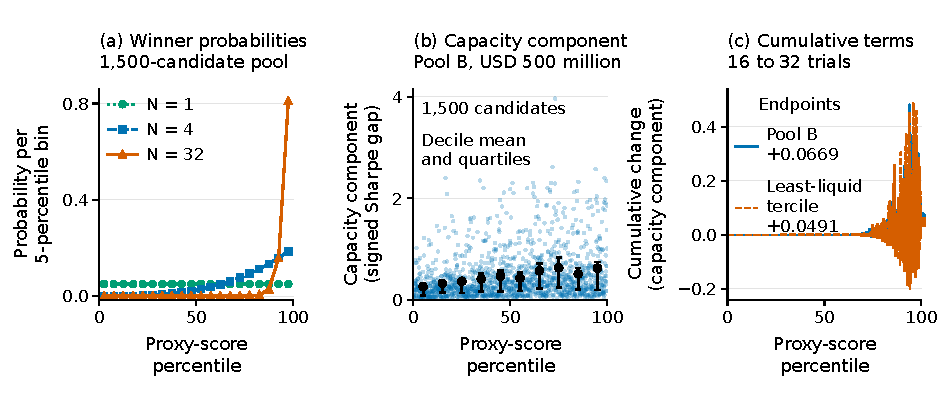
\includegraphics[width=\textwidth]{figures/finance-mechanism.pdf}
\caption{Search reweights an observed, nonmonotone gap. (a) Exact winner-rank probabilities in five-percentile bins for a 1,500-candidate pool. Higher proxy-score percentiles are better. (b) Pool B at USD 500 million: the capacity component of the signed gross-minus-net Sharpe gap for each candidate. Black marks show rank-decile means and interquartile ranges, which describe candidate spread, not uncertainty in a population mean. (c) Cumulative terms in Equation~\eqref{eq:change} for 16 to 32 trials at USD 500 million. Terms accumulate from the lowest proxy-score percentile; this reverses the best-first order in the equation but preserves the sum. Positive and negative terms offset, leaving changes $+0.0669$ in pool B and $+0.0491$ in the least-liquid tercile. These are fixed-pool calculations.}
\label{fig:mechanism}
\end{figure}

The same rank calculation exposes contrary cases (Table~\ref{tab:sensitivity}). A gap need not rise at every step just because its full-grid slope is positive. At USD 500 million, the late grid $\{8,16,32\}$ gives a capacity-component slope of $-0.0070$ in pool A. The expected gap is not monotone across the primary search budgets in pool A's four capital cells. The middle liquidity tercile also reverses the effect.

\begin{table}[htbp]
\centering
\caption{Sensitivity ranges and reversals. These settings reuse market data and candidates; cell counts do not represent independent confirmations. Walk-forward selection windows are disjoint, but earlier evaluation dates can enter later selection windows. Supporting Methods Section 4 explains the checks. The complete capital-specific rows are in \mbox{\texttt{data/finance\_additional\_checks.json}}.}
\label{tab:sensitivity}
\begin{tabular}{@{}>{\raggedright\arraybackslash}p{.18\textwidth}>{\raggedright\arraybackslash}p{.27\textwidth}>{\raggedright\arraybackslash}p{.21\textwidth}>{\raggedright\arraybackslash}p{.23\textwidth}@{}}
\toprule
Check & Variation & Capacity component at USD 500 million & Negative cases\\
\midrule
Search grids & Five grids anchored at one trial; 64 eligible pool-by-grid-by-capital cells & $[0.0172,0.0571]$ & None in anchored grids; A is $-0.0070$ on the late grid\\
Execution & Trade cap, spread, and impact assumptions & $[0.0069,0.1106]$ & None on this grid\\
Lower impact & Coefficient $0.11$ instead of $0.5$ & $[0.0052,0.0106]$ & None on this grid\\
Walk-forward & Six time periods & $[-0.0096,0.2418]$ & Seven of 72 cells across three capitals\\
Liquidity & Three retrospective terciles & Low $0.0968$; middle $-0.0279$; high $0.0334$ & Middle tercile reverses at all three capitals\\
\bottomrule
\end{tabular}

\end{table}

The primary impact coefficient is an assumption. Matching the cited temporary-impact form at 10\% participation gives a square-root coefficient of about $0.11$. With that lower coefficient, the USD 500 million capacity component remains positive but is roughly three to four times smaller. Its size is therefore sensitive to execution calibration.

Removing the single worst evaluation configuration in each cell preserves the primary signs and changes the capacity component by at most 8.6\%. This does not bound all relative changes. In pool D at USD 25 million, removing that configuration changes the near-zero net slope by about 89\%, from approximately $0.0007$ to $0.0001$. Capital ordering has limits. The capacity component increases from USD 25 million through USD 500 million in each pool. In pool A, it then falls from $0.0172$ at USD 500 million to $0.0130$ at USD 2 billion. More capital does not imply a larger signed Sharpe gap in all cases.

\section{Changing the selection score}
We compare alternative selection scores and a turnover-based candidate screen under the best-of-$N$ rule. A net-score rule uses selection-period modeled net Sharpe at an assumed capital. A calibrated turnover penalty subtracts turnover times the pool's mean selection-period gross-to-net gap divided by mean turnover. Both require the execution simulator. Table~\ref{tab:remedy} averages four pools, three assumed capitals, and three evaluation capitals at $N=32$. These 36 dependent cells use USD 25, 100, and 500 million.

\begin{table}[htbp]
\centering
\begin{tabular}{lrr}
\toprule
Selection score & Mean net Sharpe & Gain over gross\\
\midrule
Gross & $-0.501$ & $0.000$\\
Turnover decile screen & $-0.298$ & $+0.203$\\
Simulator-free penalty, $\eta_{\rm ref}=0.5$ & $-0.169$ & $+0.332$\\
Simulator-free penalty, $\eta_{\rm ref}=0.11$ & $-0.229$ & $+0.272$\\
Calibrated turnover penalty & $-0.048$ & $+0.453$\\
Net at assumed capital & $-0.071$ & $+0.430$\\
Deflated net at assumed capital & $-0.071$ & $+0.430$\\
Ex-post oracle & $+0.220$ & $+0.721$\\
\bottomrule
\end{tabular}
\caption{Changing the selection score improves mean net Sharpe, but every non-oracle mean remains negative. Each mean equally weights 36 cells at 32 trials, across four pools, three assumed capitals, and three evaluation capitals. The oracle uses evaluation outcomes and is infeasible at selection. Simulator-free penalties use full-panel universe summaries, which can include evaluation-period dates. These dependent cells do not establish future profitability.}
\label{tab:remedy}
\end{table}


The turnover decile screen removes the highest tenth of selection-period turnover before drawing $N$ candidates. Its candidate distribution therefore differs from the full-pool scoring rules. It then applies gross selection to the sampled candidates. The simulator-free penalty subtracts a cost-model coefficient times uncapped turnover; $\eta_{\rm ref}$ sets its assumed impact coefficient. The deflated-net rule uses the Deflated Sharpe Ratio to adjust for multiple trials and non-normal returns. Supporting Methods Section 4.1 gives each rule's formula and inputs.

Net-score selection improves mean net Sharpe by $0.430$ relative to gross selection. A paired joint block-bootstrap interval for the gain is $[0.192,0.723]$. The calibrated turnover penalty improves mean net Sharpe by $0.453$, with interval $[0.198,0.728]$. Each uses 1,000 replicates with a mean block length of 21. Day indices are shared across candidates, pools, and selectors. Scores and selections are recomputed. Both gains are positive in all replicates. The resulting mean levels remain negative. These are post hoc simulator comparisons of selection rules, not independent validation.

The net-score and deflated-net-score criteria produce nearly identical aggregate mean performance in this study. Nearly equal aggregate means do not imply that the two rules rank candidates identically. The result does not show that deflated Sharpe is generally ineffective. Statistical adjustment and measurement of omitted costs solve different problems.

\section{Limitations and transfer}
The strategies have no demonstrated edge. Mean candidate gross Sharpe is negative in every pool, and every tested non-oracle rule has negative mean net Sharpe on the comparison grid. The positive capacity components share one market history, and the reference joint interval for that component includes zero. Costs are modeled rather than measured from fills. The effect is smaller under lower impact. The universe is survivor-filtered, with retrospective eligibility and missing failed or delisted firms. Selection-score comparisons are post hoc. The execution model omits financing and several account constraints. Its order-dependent Sharpe decomposition is not a unique cash-cost attribution. Exact rank weights do not remove these empirical limits.

\paragraph{What would transfer.}
Lemma~\ref{lem:rank} applies to any fixed-pool best-of-$N$ search with uniform sampling without replacement and a fixed score order. The sign still depends on the outcomes attached to those ranks. Adaptive candidate generation, stopping based on observed scores, or other search laws require different probabilities. Validation loss that omits serving latency and a reward score that omits tool-use cost have the same omission structure, but we have not tested them. A test needs a stated deployment objective, the omitted term measured for each candidate, and evidence that its relation to proxy rank survives uncertainty in the selection data.

The main message is to evaluate selection on the outcome it aims to improve. In these pools, the gross-to-net gap has a positive fitted search slope, and cost-aware selection improves mean net Sharpe. Neither result establishes profitability or a stable effect on a new market path. A correction for selection noise cannot supply a cost absent from the measured objective.

\section*{Data, funding, and assistance}
The public repository at \url{https://github.com/dvgyl/when-more-search-can-worsen-deployment} contains this paper, Supporting Methods, figure data, retained finance aggregates, and verification scripts. Vendor price data are not redistributed. The package contains the retained aggregates behind the reported values, a script that checks the principal values, and the script that renders Figure~\ref{fig:mechanism}. It does not replay the raw market study. Supporting Methods identifies the original sources and reconstruction limits.

This work received no external funding. The author declares no competing interests. OpenAI Codex and Anthropic Claude assisted with research design, source analysis, derivations, code, verification, and writing. These tools are not authors. The author is responsible for the paper.
\bibliographystyle{plainnat}
\bibliography{refs}
\clearpage
\section*{NeurIPS Paper Checklist}

\begin{enumerate}

\item {\bf Claims}
    \item[] Question: Do the main claims made in the abstract and introduction accurately reflect the paper's contributions and scope?
    \item[] Answer: \answerYes{}
    \item[] Justification: The abstract and Section 1 state the fixed-pool contribution and its empirical limits. They report negative performance levels, contrary cases, and the joint interval that includes zero.
    \item[] Guidelines:
    \begin{itemize}
        \item The answer \answerNA{} means that the abstract and introduction do not include the claims made in the paper.
        \item The abstract and/or introduction should clearly state the claims made, including the contributions made in the paper and important assumptions and limitations. A \answerNo{} or \answerNA{} answer to this question will not be perceived well by the reviewers. 
        \item The claims made should match theoretical and experimental results, and reflect how much the results can be expected to generalize to other settings. 
        \item It is fine to include aspirational goals as motivation as long as it is clear that these goals are not attained by the paper. 
    \end{itemize}

\item {\bf Limitations}
    \item[] Question: Does the paper discuss the limitations of the work performed by the authors?
    \item[] Answer: \answerYes{}
    \item[] Justification: Section 6 and Supporting Methods Section 5 discuss survivor filtering, shared market history, modeled costs, exploratory comparisons, and limits on transfer. The main text also reports sensitivity to execution assumptions and search grids.
    \item[] Guidelines:
    \begin{itemize}
        \item The answer \answerNA{} means that the paper has no limitation while the answer \answerNo{} means that the paper has limitations, but those are not discussed in the paper. 
        \item The authors are encouraged to create a separate ``Limitations'' section in their paper.
        \item The paper should point out any strong assumptions and how robust the results are to violations of these assumptions (e.g., independence assumptions, noiseless settings, model well-specification, asymptotic approximations only holding locally). The authors should reflect on how these assumptions might be violated in practice and what the implications would be.
        \item The authors should reflect on the scope of the claims made, e.g., if the approach was only tested on a few datasets or with a few runs. In general, empirical results often depend on implicit assumptions, which should be articulated.
        \item The authors should reflect on the factors that influence the performance of the approach. For example, a facial recognition algorithm may perform poorly when image resolution is low or images are taken in low lighting. Or a speech-to-text system might not be used reliably to provide closed captions for online lectures because it fails to handle technical jargon.
        \item The authors should discuss the computational efficiency of the proposed algorithms and how they scale with dataset size.
        \item If applicable, the authors should discuss possible limitations of their approach to address problems of privacy and fairness.
        \item While the authors might fear that complete honesty about limitations might be used by reviewers as grounds for rejection, a worse outcome might be that reviewers discover limitations that aren't acknowledged in the paper. The authors should use their best judgment and recognize that individual actions in favor of transparency play an important role in developing norms that preserve the integrity of the community. Reviewers will be specifically instructed to not penalize honesty concerning limitations.
    \end{itemize}

\item {\bf Theory assumptions and proofs}
    \item[] Question: For each theoretical result, does the paper provide the full set of assumptions and a complete (and correct) proof?
    \item[] Answer: \answerYes{}
    \item[] Justification: Section 3 states the fixed-pool sampling and tie-order assumptions and proves Lemma~\ref{lem:rank}. It also gives the two-candidate identification argument; Supporting Methods Section 4 proves the stated score-error bound.
    \item[] Guidelines:
    \begin{itemize}
        \item The answer \answerNA{} means that the paper does not include theoretical results. 
        \item All the theorems, formulas, and proofs in the paper should be numbered and cross-referenced.
        \item All assumptions should be clearly stated or referenced in the statement of any theorems.
        \item The proofs can either appear in the main paper or the supplemental material, but if they appear in the supplemental material, the authors are encouraged to provide a short proof sketch to provide intuition. 
        \item Inversely, any informal proof provided in the core of the paper should be complemented by formal proofs provided in appendix or supplemental material.
        \item Theorems and Lemmas that the proof relies upon should be properly referenced. 
    \end{itemize}

\item {\bf Experimental result reproducibility}
    \item[] Question: Does the paper fully disclose all the information needed to reproduce the main experimental results of the paper to the extent that it affects the main claims and/or conclusions of the paper (regardless of whether the code and data are provided or not)?
    \item[] Answer: \answerNo{}
    \item[] Justification: Supporting Methods Sections 1--4 specify the procedure, but the exact raw-data snapshot, candidate return arrays, complete simulator, and original environment are not supplied. The initial ticker list also has incomplete provenance, so the aggregate package does not permit full reproduction.
    \item[] Guidelines:
    \begin{itemize}
        \item The answer \answerNA{} means that the paper does not include experiments.
        \item If the paper includes experiments, a \answerNo{} answer to this question will not be perceived well by the reviewers: Making the paper reproducible is important, regardless of whether the code and data are provided or not.
        \item If the contribution is a dataset and\slash or model, the authors should describe the steps taken to make their results reproducible or verifiable. 
        \item Depending on the contribution, reproducibility can be accomplished in various ways. For example, if the contribution is a novel architecture, describing the architecture fully might suffice, or if the contribution is a specific model and empirical evaluation, it may be necessary to either make it possible for others to replicate the model with the same dataset, or provide access to the model. In general. releasing code and data is often one good way to accomplish this, but reproducibility can also be provided via detailed instructions for how to replicate the results, access to a hosted model (e.g., in the case of a large language model), releasing of a model checkpoint, or other means that are appropriate to the research performed.
        \item While NeurIPS does not require releasing code, the conference does require all submissions to provide some reasonable avenue for reproducibility, which may depend on the nature of the contribution. For example
        \begin{enumerate}
            \item If the contribution is primarily a new algorithm, the paper should make it clear how to reproduce that algorithm.
            \item If the contribution is primarily a new model architecture, the paper should describe the architecture clearly and fully.
            \item If the contribution is a new model (e.g., a large language model), then there should either be a way to access this model for reproducing the results or a way to reproduce the model (e.g., with an open-source dataset or instructions for how to construct the dataset).
            \item We recognize that reproducibility may be tricky in some cases, in which case authors are welcome to describe the particular way they provide for reproducibility. In the case of closed-source models, it may be that access to the model is limited in some way (e.g., to registered users), but it should be possible for other researchers to have some path to reproducing or verifying the results.
        \end{enumerate}
    \end{itemize}

\item {\bf Open access to data and code}
    \item[] Question: Does the paper provide open access to the data and code, with sufficient instructions to faithfully reproduce the main experimental results, as described in supplemental material?
    \item[] Answer: \answerNo{}
    \item[] Justification: The linked repository provides retained aggregates, figure inputs, and verification scripts. It does not provide the raw prices, candidate return arrays, complete simulator, or environment needed to reproduce the market experiments.
    \item[] Guidelines:
    \begin{itemize}
        \item The answer \answerNA{} means that paper does not include experiments requiring code.
        \item Please see the NeurIPS code and data submission guidelines (\url{https://neurips.cc/public/guides/CodeSubmissionPolicy}) for more details.
        \item While we encourage the release of code and data, we understand that this might not be possible, so \answerNo{} is an acceptable answer. Papers cannot be rejected simply for not including code, unless this is central to the contribution (e.g., for a new open-source benchmark).
        \item The instructions should contain the exact command and environment needed to run to reproduce the results. See the NeurIPS code and data submission guidelines (\url{https://neurips.cc/public/guides/CodeSubmissionPolicy}) for more details.
        \item The authors should provide instructions on data access and preparation, including how to access the raw data, preprocessed data, intermediate data, and generated data, etc.
        \item The authors should provide scripts to reproduce all experimental results for the new proposed method and baselines. If only a subset of experiments are reproducible, they should state which ones are omitted from the script and why.
        \item At submission time, to preserve anonymity, the authors should release anonymized versions (if applicable).
        \item Providing as much information as possible in supplemental material (appended to the paper) is recommended, but including URLs to data and code is permitted.
    \end{itemize}

\item {\bf Experimental setting/details}
    \item[] Question: Does the paper specify all the training and test details (e.g., data splits, hyperparameters, how they were chosen, type of optimizer) necessary to understand the results?
    \item[] Answer: \answerYes{}
    \item[] Justification: Section 4 gives the data periods, candidate models, selection score, and execution assumptions. Supporting Methods Sections 1--4 give feature formulas, configuration grids and seeds, fitting details, timing, portfolio rules, and resampling settings.
    \item[] Guidelines:
    \begin{itemize}
        \item The answer \answerNA{} means that the paper does not include experiments.
        \item The experimental setting should be presented in the core of the paper to a level of detail that is necessary to appreciate the results and make sense of them.
        \item The full details can be provided either with the code, in appendix, or as supplemental material.
    \end{itemize}

\item {\bf Experiment statistical significance}
    \item[] Question: Does the paper report error bars suitably and correctly defined or other appropriate information about the statistical significance of the experiments?
    \item[] Answer: \answerYes{}
    \item[] Justification: Sections 4.3 and 5 report percentile intervals from 1,000 stationary block bootstrap replicates. Supporting Methods Section 4 states the shared day-index scheme, separate period resampling, block lengths, seeds, and conditional interpretation.
    \item[] Guidelines:
    \begin{itemize}
        \item The answer \answerNA{} means that the paper does not include experiments.
        \item The authors should answer \answerYes{} if the results are accompanied by error bars, confidence intervals, or statistical significance tests, at least for the experiments that support the main claims of the paper.
        \item The factors of variability that the error bars are capturing should be clearly stated (for example, train/test split, initialization, random drawing of some parameter, or overall run with given experimental conditions).
        \item The method for calculating the error bars should be explained (closed form formula, call to a library function, bootstrap, etc.)
        \item The assumptions made should be given (e.g., Normally distributed errors).
        \item It should be clear whether the error bar is the standard deviation or the standard error of the mean.
        \item It is OK to report 1-sigma error bars, but one should state it. The authors should preferably report a 2-sigma error bar than state that they have a 96\% CI, if the hypothesis of Normality of errors is not verified.
        \item For asymmetric distributions, the authors should be careful not to show in tables or figures symmetric error bars that would yield results that are out of range (e.g., negative error rates).
        \item If error bars are reported in tables or plots, the authors should explain in the text how they were calculated and reference the corresponding figures or tables in the text.
    \end{itemize}

\item {\bf Experiments compute resources}
    \item[] Question: For each experiment, does the paper provide sufficient information on the computer resources (type of compute workers, memory, time of execution) needed to reproduce the experiments?
    \item[] Answer: \answerNo{}
    \item[] Justification: The paper does not report the original hardware, memory use, execution times, or total research compute. The aggregate verification scripts do not recover these quantities.
    \item[] Guidelines:
    \begin{itemize}
        \item The answer \answerNA{} means that the paper does not include experiments.
        \item The paper should indicate the type of compute workers CPU or GPU, internal cluster, or cloud provider, including relevant memory and storage.
        \item The paper should provide the amount of compute required for each of the individual experimental runs as well as estimate the total compute. 
        \item The paper should disclose whether the full research project required more compute than the experiments reported in the paper (e.g., preliminary or failed experiments that didn't make it into the paper). 
    \end{itemize}

\item {\bf Code of ethics}
    \item[] Question: Does the research conducted in the paper conform, in every respect, with the NeurIPS Code of Ethics \url{https://neurips.cc/public/EthicsGuidelines}?
    \item[] Answer: \answerYes{}
    \item[] Justification: The author has reviewed the NeurIPS Code of Ethics and confirms that this research conforms to it.
    \item[] Guidelines:
    \begin{itemize}
        \item The answer \answerNA{} means that the authors have not reviewed the NeurIPS Code of Ethics.
        \item If the authors answer \answerNo, they should explain the special circumstances that require a deviation from the Code of Ethics.
        \item The authors should make sure to preserve anonymity (e.g., if there is a special consideration due to laws or regulations in their jurisdiction).
    \end{itemize}

\item {\bf Broader impacts}
    \item[] Question: Does the paper discuss both potential positive societal impacts and negative societal impacts of the work performed?
    \item[] Answer: \answerNo{}
    \item[] Justification: The paper explains the risk of selection scores that omit deployment costs and states that the strategies have no demonstrated trading advantage. It does not give a full assessment of positive and negative societal impacts.
    \item[] Guidelines:
    \begin{itemize}
        \item The answer \answerNA{} means that there is no societal impact of the work performed.
        \item If the authors answer \answerNA{} or \answerNo, they should explain why their work has no societal impact or why the paper does not address societal impact.
        \item Examples of negative societal impacts include potential malicious or unintended uses (e.g., disinformation, generating fake profiles, surveillance), fairness considerations (e.g., deployment of technologies that could make decisions that unfairly impact specific groups), privacy considerations, and security considerations.
        \item The conference expects that many papers will be foundational research and not tied to particular applications, let alone deployments. However, if there is a direct path to any negative applications, the authors should point it out. For example, it is legitimate to point out that an improvement in the quality of generative models could be used to generate Deepfakes for disinformation. On the other hand, it is not needed to point out that a generic algorithm for optimizing neural networks could enable people to train models that generate Deepfakes faster.
        \item The authors should consider possible harms that could arise when the technology is being used as intended and functioning correctly, harms that could arise when the technology is being used as intended but gives incorrect results, and harms following from (intentional or unintentional) misuse of the technology.
        \item If there are negative societal impacts, the authors could also discuss possible mitigation strategies (e.g., gated release of models, providing defenses in addition to attacks, mechanisms for monitoring misuse, mechanisms to monitor how a system learns from feedback over time, improving the efficiency and accessibility of ML).
    \end{itemize}

\item {\bf Safeguards}
    \item[] Question: Does the paper describe safeguards that have been put in place for responsible release of data or models that have a high risk for misuse (e.g., pre-trained language models, image generators, or scraped datasets)?
    \item[] Answer: \answerNA{}
    \item[] Justification: The release contains retained aggregates, figure inputs, and verification scripts, with no trained models or raw price records. These assets do not present the high-risk release cases described in this question.
    \item[] Guidelines:
    \begin{itemize}
        \item The answer \answerNA{} means that the paper poses no such risks.
        \item Released models that have a high risk for misuse or dual-use should be released with necessary safeguards to allow for controlled use of the model, for example by requiring that users adhere to usage guidelines or restrictions to access the model or implementing safety filters. 
        \item Datasets that have been scraped from the Internet could pose safety risks. The authors should describe how they avoided releasing unsafe images.
        \item We recognize that providing effective safeguards is challenging, and many papers do not require this, but we encourage authors to take this into account and make a best faith effort.
    \end{itemize}

\item {\bf Licenses for existing assets}
    \item[] Question: Are the creators or original owners of assets (e.g., code, data, models), used in the paper, properly credited and are the license and terms of use explicitly mentioned and properly respected?
    \item[] Answer: \answerNo{}
    \item[] Justification: Supporting Methods Section 1 credits Yahoo Finance and gives its data endpoint. The paper does not establish all applicable asset licenses and terms of use, and vendor price records are not redistributed.
    \item[] Guidelines:
    \begin{itemize}
        \item The answer \answerNA{} means that the paper does not use existing assets.
        \item The authors should cite the original paper that produced the code package or dataset.
        \item The authors should state which version of the asset is used and, if possible, include a URL.
        \item The name of the license (e.g., CC-BY 4.0) should be included for each asset.
        \item For scraped data from a particular source (e.g., website), the copyright and terms of service of that source should be provided.
        \item If assets are released, the license, copyright information, and terms of use in the package should be provided. For popular datasets, \url{paperswithcode.com/datasets} has curated licenses for some datasets. Their licensing guide can help determine the license of a dataset.
        \item For existing datasets that are re-packaged, both the original license and the license of the derived asset (if it has changed) should be provided.
        \item If this information is not available online, the authors are encouraged to reach out to the asset's creators.
    \end{itemize}

\item {\bf New assets}
    \item[] Question: Are new assets introduced in the paper well documented and is the documentation provided alongside the assets?
    \item[] Answer: \answerYes{}
    \item[] Justification: The aggregate package includes a README, reproduction details, field definitions, a hashed data manifest, and verification and figure commands. These documents state that raw-study reproduction is unavailable and assert no new license grant.
    \item[] Guidelines:
    \begin{itemize}
        \item The answer \answerNA{} means that the paper does not release new assets.
        \item Researchers should communicate the details of the dataset\slash code\slash model as part of their submissions via structured templates. This includes details about training, license, limitations, etc. 
        \item The paper should discuss whether and how consent was obtained from people whose asset is used.
        \item At submission time, remember to anonymize your assets (if applicable). You can either create an anonymized URL or include an anonymized zip file.
    \end{itemize}

\item {\bf Crowdsourcing and research with human subjects}
    \item[] Question: For crowdsourcing experiments and research with human subjects, does the paper include the full text of instructions given to participants and screenshots, if applicable, as well as details about compensation (if any)? 
    \item[] Answer: \answerNA{}
    \item[] Justification: The study uses historical equity price and volume records. It includes no crowdsourcing or research with human participants.
    \item[] Guidelines:
    \begin{itemize}
        \item The answer \answerNA{} means that the paper does not involve crowdsourcing nor research with human subjects.
        \item Including this information in the supplemental material is fine, but if the main contribution of the paper involves human subjects, then as much detail as possible should be included in the main paper. 
        \item According to the NeurIPS Code of Ethics, workers involved in data collection, curation, or other labor should be paid at least the minimum wage in the country of the data collector. 
    \end{itemize}

\item {\bf Institutional review board (IRB) approvals or equivalent for research with human subjects}
    \item[] Question: Does the paper describe potential risks incurred by study participants, whether such risks were disclosed to the subjects, and whether Institutional Review Board (IRB) approvals (or an equivalent approval/review based on the requirements of your country or institution) were obtained?
    \item[] Answer: \answerNA{}
    \item[] Justification: The study includes no human participants or crowdsourcing. No participant consent or institutional review board approval is claimed.
    \item[] Guidelines:
    \begin{itemize}
        \item The answer \answerNA{} means that the paper does not involve crowdsourcing nor research with human subjects.
        \item Depending on the country in which research is conducted, IRB approval (or equivalent) may be required for any human subjects research. If you obtained IRB approval, you should clearly state this in the paper. 
        \item We recognize that the procedures for this may vary significantly between institutions and locations, and we expect authors to adhere to the NeurIPS Code of Ethics and the guidelines for their institution. 
        \item For initial submissions, do not include any information that would break anonymity (if applicable), such as the institution conducting the review.
    \end{itemize}

\item {\bf Declaration of LLM usage}
    \item[] Question: Does the paper describe the usage of LLMs if it is an important, original, or non-standard component of the core methods in this research? Note that if the LLM is used only for writing, editing, or formatting purposes and does \emph{not} impact the core methodology, scientific rigor, or originality of the research, declaration is not required.
    \item[] Answer: \answerYes{}
    \item[] Justification: The Data, funding, and assistance statement discloses assistance from OpenAI Codex and Anthropic Claude with research design, source analysis, derivations, code, verification, and writing. It assigns responsibility for the paper to the author.
    \item[] Guidelines:
    \begin{itemize}
        \item The answer \answerNA{} means that the core method development in this research does not involve LLMs as any important, original, or non-standard components.
        \item Please refer to our LLM policy in the NeurIPS handbook for what should or should not be described.
    \end{itemize}

\end{enumerate}

\end{document}
